%!TEX root = paper.tex
\section{BLE Hardware Imperfections}
\label{sec:background}

In this section, we explain different aspects of bluetooth low energy protocol. We first explain both physical and medium access control layer of BLE communication protocol that is used for advertising. Next, we present the most popular hardware architecture used for designing BLE chipsets and explain the possible hardware signatures which could be used for RF fingerprinting. 

\subsection{Bluetooth Low Energy Communication Protocol}

\begin{comment}
\begin{figure*}
    \centering
    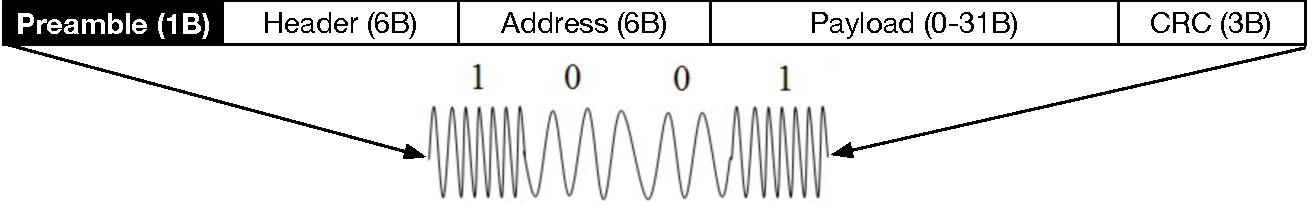
\includegraphics[width = \linewidth]{plots/advertisingpacket.pdf} \label{figure2}
    \caption{BLE Packet Format}
    \label{fig:2}
    \end{figure*}
\end{comment}



Bluetooth Low Energy (BLE) is a wireless personal area network topology, designed particularly for short-range communication, within small clusters of devices (known as piconets). It achieves low power consumption by using a low transmission power for active communication, therefore are energy efficient.

\paragraph{BLE Physical-Layer} BLE operates in the 2.4 GHz ISM band, with 40 channels each channel is separated with 2 MHz channel spacing. Of these 3 channels are designated advertisement channels, and the remaining 37 data channels. BLE uses Gaussian Frequency Shift Keying as the modulation scheme, where in, a device transmits one frequency for bit 0 and sends another frequency for bit 1. These frequencies are typically $\pm f_d$ around the center frequency, with a typical value of 250 KHz. The frequency deviation in this case be denoted as either $f_d$ (we use $f_d$ in the rest of the paper). Finally a Gaussian pulse shaping filter is applied on the signal to smoothen the transitions between different frequencies, resulting in a band-limited signal. The bandwidth of BLE communication is typically less than 1 MHz, which is 20 $\times$ lower than the WiFi bandwidth. 

%In Figure~\ref{fig:idealgfsk} we show an example of the instantaneuous frequency GFSK-modulated signal, with a frequency deviation of 250 KHz.
%
%An effect of Gaussian smoothing is that the frequency cannot catch the intended frequency whenever there are 010 or 101 sequences. 
\begin{comment}
\begin{figure}
\centering
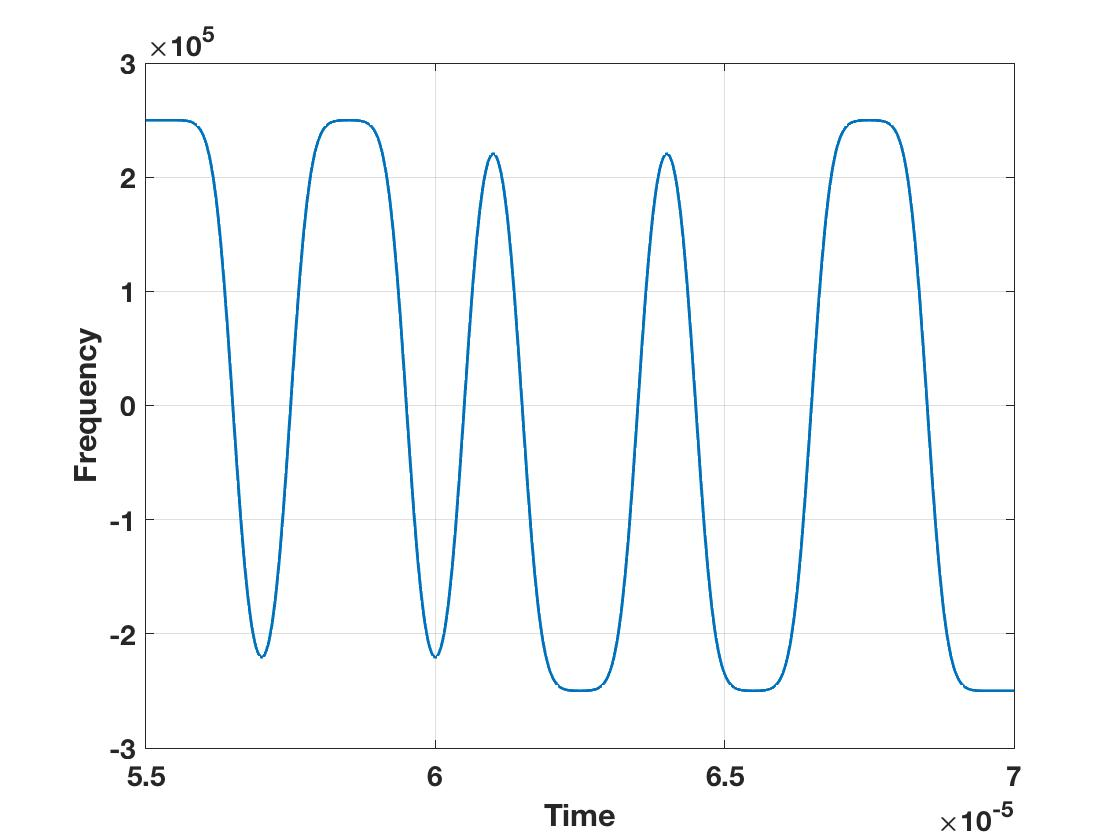
\includegraphics[width = \linewidth]{plots/sample_freq.jpg} \label{figure1}
\caption{Sample of an Ideal Instantaneous Frequency of GFSK Modulation}
\label{fig:idealgfsk}
\end{figure}
\end{comment}

\paragraph{BLE Advertisement packets} BLE devices utilize advertisement packets to indicate their presence to other devices in the vicinity. Advertisement packets are short packets (at most 376 microseconds) which are frequently sent. The packet length is shorter to save on energy and is typically 1/4 of the WiFi packets. Advertisement packets include an 8-bit preamble, which is 10 $\times$ smaller compared to the WiFi preamble design. Furthermore, the packet consists of a unique 48-bit identifier as advertising address (typically the hardware MAC address of the radio), which is transmitted as part of the payload. Since every packet contains the unique address, potential for tracking the device became a concern. To alleviate this, Bluetooth SIG introduced address randomization (as discussed in Section~\ref{sec:motivation}). Finally, the complete advertising payload is appended with the CRC and is whitened or scrambled. 

The receiver to decode the data only observes the frequency shift of the received data. It notes the zero crossing of the frequency to decode the bit either to 0 or 1. Thus simplifying the decoder design as well, compared to multi-carrier WiFi modulation. 

\subsection{BLE Chipset Design \& Source of Hardware Imperfections}
In this subsection, we present the design of the chipsets capable of sending BLE advertisement packets. The most pervasive BLE transmitter architecture is a WiFi/BLE combo chipset that is used in smartphones, tablets, laptops, Apple watches and almost any device that supports both Wi-Fi and BLE. BLE beacons emitted from these chipsets randomize their MAC address, making the identification through MAC address impossible. This is where our RF identification attacks comes into play. The other kind of BLE transmitter architecture is a BLE-only chipset that is used in a few products such as fitbit which is supposed to only support BLE. Interestingly, our observations show that the devices using these BLE-only chipsets do not randomize their MAC address and exploit a static MAC address. Since these devices use a static MAC address, one can identify the device simply using its MAC address and there is no need to employ a more complicated RF identification attack. As a result, we only develop and deploy our attack for the target devices that has the Wi-Fi/BLE combo chipset. In other words, when we want to decide whether a device is our target, we first check the MAC address of the device against the MAC address of the target that we have observed before. If the MAC address was the same, then we can identify it based on its MAC address and if the MAC address was different, we can identify the device using its RF fingerprints.

To deploy our RF identification attack, we should estimate the imperfections or uniqueness of the RF signal generated by different devices. Designing an algorithm to capture and extract these imperfections from signals, requires the knowledge of possible hardware imperfection sources in the RF chain. These imperfections originate from the analog components in the RF chain. In the rest of this section, we elaborate upon the Wi-Fi/BLE combo chipset architecture and the hardware imperfections generated by these chipsets that might be useful to uniquely identify a device.


%\subsubsection{WiFi/BLE Combo Chipsets}
\paragraph{WiFi/BLE Combo Chipsets}
WiFi chipsets require generation of complex multi-carrier modulation waveform, which popularly uses the I/Q modulation architecture shown in Figure.~\ref{fig:iq_arch}, where in, I (real) and Q (imaginary) parts of the waveform are generated by the digital baseband. The real and imaginary parts of the signal are eventually mixed at the carrier frequency ($f_c$), where real part is multiplied cosine ($cos(2\pi f_c t$) of the carrier frequency and vice versa for imaginary part. In order to save cost of RF hardware, high power devices (e.g. smartphones) are equipped with combo chips which have both BLE and WiFi digital baseband, and they share the IQ front-end as shown in Figure.~\ref{fig:iq_arch}. Thus simplifying the smartphone design, and optimizing die size and smartphone area.

\paragraph{Imperfections of the Combo chipsets}

The hardware imperfections in this kind of hardware architecture, includes carrier frequency offset (CFO) and IQ imperfections (which itself consists of IQ offset and IQ imbalance). CFO is the error in the carrier frequency fed to the mixer and is caused by the oscillator on the chip. The crystal and the tolerance of oscillators yields unique CFO even the devices from the same make and model. 
IQ offset is caused when center carrier leaks into the signal or when baseband signal has a DC offset. This can add a fixed complex term to the I and Q sample (shift the center of constellation). IQ imbalance occurs because of mismatch between parallel analog components of RF chain in I (in-phase) and Q (quadrature) signal path. This makes the phase and amplitude of I and Q path asymmetric. These hardware imperfections have been demonstrated to be the most important characteristics for building RF fingerprinting systems for WiFi devices. As a result, we can take advantage of these previously explored hardware imperfections to build our physical layer attack on BLE devices. However, as discussed in section~\ref{sec:motivation}, unlike WiFi estimating these imperfection for BLE devices is extremely challenging, and there is no existing technique for estimating the mentioned imperfections for BLE devices with the granularity and accuracy which is needed for the task of device identification. Consequently, in subsection~\ref{sec:methodology1}, we develop a new algorithm to estimate these imperfections accurately and robustly.

%A natural question is how can measure these quantities using the BLE transmissions. Decoding the simple GFSK modulation which is used in BLE,is not affected by the aforementioned imperfections severely. Therefore,there has not been any attempt on measuring these impairments accurately for a BLE or Bluetooth signal. Also, using the same techniques for estimating impairments as WiFi, will result in a much lower accuracy of estimation because of having a narrowband (without subcarrier), with a very short preamble 8 bits (i.e. 8 microseconds). Specifically, in order to estimate the carrier frequency offset accurately to sub 100 Hz accuracy would requires 100's of usec of narrow bandwidth signal  or 10's usec of wide-bandwidth signal. However, the preamble of the BLE falls short of meeting this requirement. 

%Measuring these hardware imperfections is an unavoidable stage in decoding WiFi packets since it can significantly affect the decoding error if the receiver does not compensate them. As a result, measuring these imperfection has been heavily researched for WiFi signals. More than that, the standard WiFi protocol offers facilities to make the estimation of these imperfections easy and accurate (e.g. LTF, subcarriers, channel state information (CSI)). 
 

%For instance, we employed the technique that is used in Bluetooth test equipments which exploits the preamble to estimate CFO [CITE]. That is,simply we take the average of frequencies in the preamble. Since preamble is an 8-bit sequence of consecutive 0 and 1, the frequency of preamble is symmetric. Therefore, ideally the average of the frequencies in preamble must be 0. If there exists CFO, this average will be an estimate of CFO. However, this estimation is not precise and robust enough as it only relies on a an 8-microsecond preamble. The resulting standard deviation of the measured CFO was 1.5 KHz (we averaged the CFO standard deviation across 20 different devices). This standard deviation is huge for performing the task of RF fingeprinting and will end up in low accuracy of identifying devices based on RF fingerprints. We also tried the MINMAX algorithm described in [CITE] but it yielded even worse standard deviation.


\begin{figure}[t!]
    \centering
    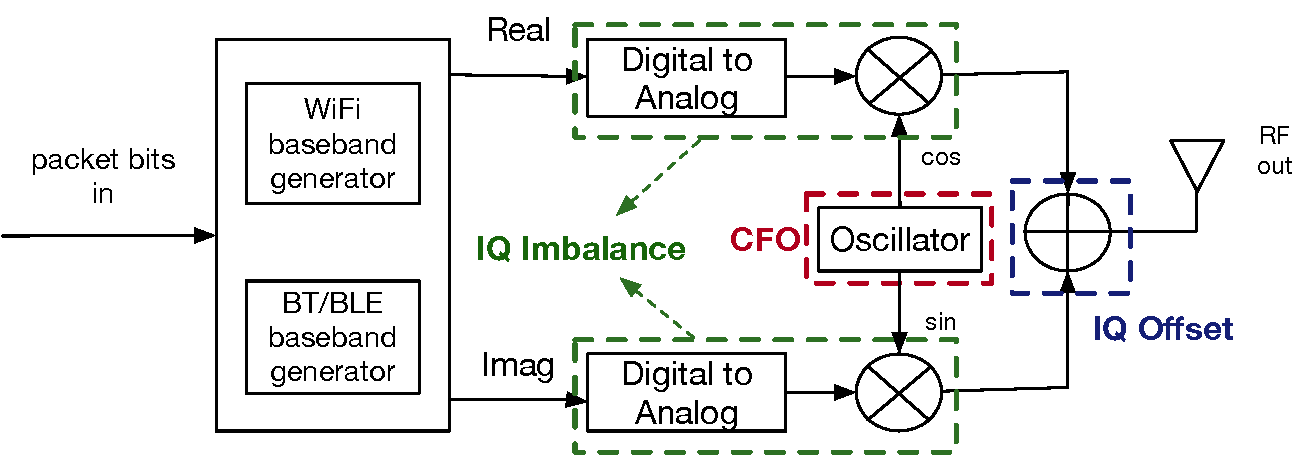
\includegraphics[width = \linewidth]{plots/IQchain.pdf} 
    \caption{Architecture of WiFi/BLE combo chipsets}
    \label{fig:iq_arch}
\end{figure}


% \begin{figure*}
% \centering
% \begin{minipage}{0.45\textwidth}
% \centering
% 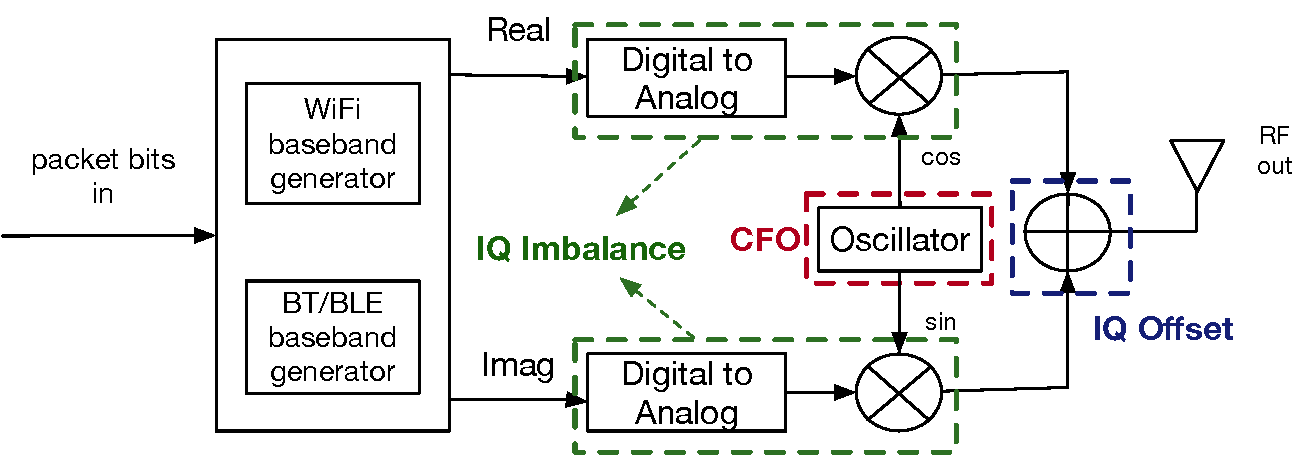
\includegraphics[width=\linewidth]{plots/IQchain.pdf}
% \caption{
% \label{fig:iq_arch}
% Architecture of WiFi/BLE combo chipsets
% }
% \end{minipage}
% \end{figure*}
%
%\hspace{0.02\textwidth}
% %
% \begin{minipage}{0.45\textwidth}
% \centering
% 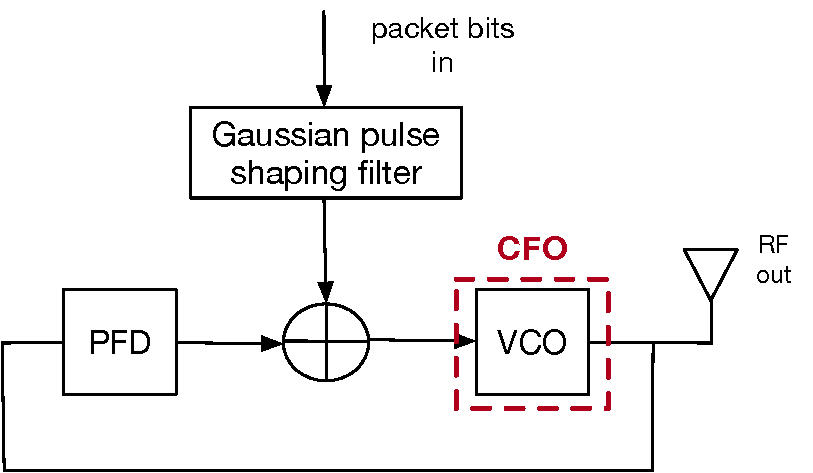
\includegraphics[width=0.75\linewidth]{plots/dpll.pdf}
% \caption{
% \label{fig:dpll}
% Architecture of low-power BLE-only chipsets
% }
% \end{minipage}
% \label{figure1}
% \end{figure*}

% \subsubsection{BLE-only Chipsets}
% We discovered that not all BLE transmitters use the combo architecture. Interestingly, the devices that are only supposed to support BLE (such as fitbit) or other low power technologies, employ a fundamentally different architecture without having I/Q modulation and mixer. As shown in Figure~\ref{fig:dpll} , in such architecture, the modulated samples are directly fed to a Phase-Locked Loop (PLL) which generates the required frequencies by moving the carrier frequency up and down to create GFSK waveform. There exist different designs for such an architecture. For instance, in some of them, the loop will be opened once the channel frequency is fixed and the GFSK frequencies are generated in an open-loop VCO~\cite{?}. In some other, digital modulated samples drive a DCO which adjusts the frequency using capacitors and a $\Sigma \Delta$ modulator. However, the common characteristic in all these designs is that the frequency of 1's and 0's is controlled by an analog component.


% \paragraph{Imperfections of the BLE-only Chipsets}
% As mentioned earlier, we discovered IQ modulation does not exist in BLE-only chip design . Therefore, unlike the former architecture, we are deprived from the two impairments, IQ imbalance and IQ offset. Instead, the imperfections in the PLL could be a rich source for distinguishing different devices. Depending on the design, these imperfections could have different sources such as loop filter, VCO, capacitors, etc. However, the key fact about this kind of imperfection is that, no matter what the source is, it will represents its effect in the frequencies generated by the transmitter since PLL is responsible for outputting the frequency of GFSK signal in this architecture. To our knowledge, this kind of imperfection has never been introduced in prior RF fingerpriting works.

%  A consequence of the above is that there is not a specific source of impairment, we can profile to characterize the uniqueness of the BLE device. Instead we observe that in order to take advantage of the new sources of imperfection, we must profile the frequencies generated by the transmitter, as all these impairments would affect how the frequencies are generated in the time-series of the packet generation. Therefore, we need a new robust technique which profiles frequencies generated by a transmitter while preserving any and all information that can be used for identification. Specifically, First, we need a new representation of the information in which all the information about identification is preserved. Second, we need a technique which can extract the parameters which are unique for each BLE device, as we do not have the specific architecture a BLE device belongs to (Section~\ref{sec:methodology2}). 




 %As we have two major category of transmitter architecture for BLE transmitters, we must derive algorithms to capture the impairments existing in both kinds of architecture.


%The immediate solution for profiling frequency, is using Fourier transform. However, there is a major problem with using Fourier transform. BLE advertisements sent by a device, quite often have a fixed payload data (or at most a very small set of different payload data). As a result, during a MAC address lifetime, the whitened packet sent from a device is fixed. Consequently, we found that if we train a machine learning model on the signal or Fourier transform of the signal, it will simply ignore extracting those slight hardware imperfections since it can simply distinguish devices by only using their packet bit sequence. However, in the next MAC address lifetime, the change in MAC address (and possibly other parts of the payload) completely changes the packet after whitening. Consequently, we cannot identify the device anymore because instead of any hardware imperfections, it has just learnt to distinguish the devices based on their packet sequence. Thus, using Fourier transform does not work for our problem.
 



\begin{comment}
\subsubsection{Most Personal Devices Are Beaconing}
Low power consumption feature of BLE technology makes it a suitable solution to many applications from retail industry to personal use cases. Medicine, fitness tracking, retail, smart tags, ,smart cars, education, social networks, Nearby technology and Apple's Continuity protocol are only a number of rapidly growing use cases of BLE technology in people's lives. However, to enable such applications, these smart devices including smartphones, smartwatches earphones, Tablets, fitness trackers and smart tags attached properties are frequently sending BLE packets to communicate with each other. Beaconing all the time is equivalent to announcing the presence of the device to the world and this may eventually lead to announcing the presence of a person as one can correspond the devices to people by using other information from the world. Consequently, a malicious attacker may sniff the frequently-sent BLE packets from a device and attempt to track or detect the presence of someone. Becker \textit{et al.} \cite{Iphonetracking_becker} conduct a study on how frequently some commonly used devices send BLE packets. For instance, they claim that MacOS and iOS device advertise their presence up to two advertising events per second which was also verified by our study on iPhones. 

\subsubsection{MAC Address Randomization}
Given the abundant number of packets sent by a typicol personal device, keeping MAC address unchanged can cause privacy issues as an attacker may listen to the MAC address and obtain private information of the user. One the most important privacy issues is that the attacker can detect the presence of a device or even track it by listening to its MAC address. To overcome this issue, BLE protocol suggest randomizing MAC address after a while. The suggested time interval after which the device changes its MAC address is 15 minutes. However, this is the suggested time by BLE protocol and is not a requirement. Manufacturers may choose different time periods or even ignore MAC address randomization in their implementation.
Becker \textit{et al.} \cite{Iphonetracking_becker} also include some information about how often different devices change their MAC address. A summary of their study is presented in table \ref{table:1}. As mentioned earlier, macOS and iOS devices send advertisement packets roughly twice a second. Therefore, even with ignoring the data packets, macOS and iOS devices send approximately 2400 advertisement packets with a fixed MAC address given the 20-minute address lifetime of these devices. We will show that this amount of packets is more than enough for the attacker to build a reliable profile for those devices to track them.

\begin{table}[t!]                           
\centering
%!TEX root = ../paper.tex
\begin{tabular}{|c|c|}
	\hline
     \textbf{Device Type}    &   \textbf{Address Life}                
     \\ \hline
     macOS, iOS &  20 min             
     \\ \hline          
     Android    &   15-45 min  
     \\ \hline
     Windows 10          &   16 min           
     \\ \hline
     Microsoft Surface          &   16 min
     \\ \hline
     Fitbit Charge          &   static
     \\ \hline
\end{tabular}
\caption{MAC Address Lifetime}
\label{table:1}
\end{table}
\end{comment}






